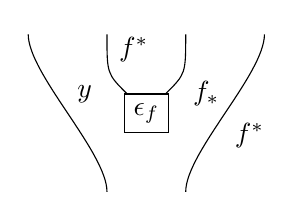
\begin{tikzpicture}[baseline=(current bounding box.center),]
\path coordinate[] (tikzsd_internal_pos_0_0) at (0.0,0.0);
\path coordinate[] (tikzsd_internal_pos_0_1) at (1.0,0.0);
\path coordinate[] (tikzsd_internal_pos_0_2) at (2.0,0.0);
\path coordinate[] (tikzsd_internal_pos_0_3) at (3.0,0.0);
\path coordinate[] (tikzsd_internal_pos_1_0) at (1.0,-2.0);
\path coordinate[] (tikzsd_internal_pos_1_1) at (2.0,-2.0);

\path node[,draw,] (tikzsd_internal_nt_node_0_0) at (1.5,-1.0) {$\epsilon_f$};

\path [draw] (tikzsd_internal_pos_0_0) ..controls(0.0,-0.5)and(1.0,-1.5)..(tikzsd_internal_pos_1_0) node[pos=0.5,auto,] {$y$};
\path [draw] (tikzsd_internal_pos_0_1) ..controls(1.0,-0.5)..(tikzsd_internal_nt_node_0_0) node[pos=0.5,auto,] {$f^\ast$};
\path [draw] (tikzsd_internal_pos_0_2) ..controls(2.0,-0.5)..(tikzsd_internal_nt_node_0_0) node[pos=0.5,auto,] {$f_\ast$};
\path [draw] (tikzsd_internal_pos_0_3) ..controls(3.0,-0.5)and(2.0,-1.5)..(tikzsd_internal_pos_1_1) node[pos=0.5,auto,] {$f^\ast$};
\end{tikzpicture}